 \clearpage
 %%%%%%%%%%%%%%%%%%%%%%%%%%%%%%%%%%%%%%%%%%%%%%%%%%%%%%%%%%%%%%%%%%%%%%%%%%%%%%%%%
 %%        %%%        %%%        %%%        %%%        %%%         %%%  %%%%  %%%
 %%  %%%%%%%%%  %%%%%%%%%  %%%%%%%%%%%%  %%%%%%%%%  %%%%%%  %%%%%  %%%    %%  %%%
 %%        %%%        %%%  %%%%%%%%%%%%  %%%%%%%%%  %%%%%%  %%%%%  %%%  %  %  %%%
 %%%%%%%%  %%%  %%%%%%%%%  %%%%%%%%%%%%  %%%%%%%%%  %%%%%%  %%%%%  %%%  %%    %%%
 %%        %%%        %%%        %%%%%%  %%%%%%        %%%         %%%  %%%   %%%
 %%%%%%%%%%%%%%%%%%%%%%%%%%%%%%%%%%%%%%%%%%%%%%%%%%%%%%%%%%%%%%%%%%%%%%%%%%%%%%%%%
 \section{TGraph}
 \ROOT を使ってx座標及びy座標を与えてグラフを描くことが大いに考えられる。
 \ROOT では\verb|TGraph|を使うことで実現できる。
 
 
\subsection{ファイルから読み込んでグラフ化する}
シンチレータと光電子増倍管を組み合わせた検出器を考える。
光電子増倍管からの信号にある閾値を設け、
光電子増倍管に印加する電圧を変化させて単位時間あたりにどれだけの収量が得られたかを測定した実験を考える。
この時、下記のような形式のデータファイルをきっと作ることだろう。
 \begin{itembox}{\texttt{plateaudata.plt}}
\begin{verbatim}
	# HV[V]  Counts[c/min]
1400  3
1450  1
1500  2
1550  10
1600  14
1650  20
1700  80
1750  250
1800  600
1850  900
1900  1000
1950  1050
2000  1060
2050  1090
2100  1095
2150  1100
2200  1105
2250  1108
2300  1109
2350  1105
2400  1110
2450  1120
2500  1150
2550  1240
2600  1350
2650  1505
2700  1700
\end{verbatim}
 \end{itembox}
\verb|plateaudata.plt|をプロットする方法はいくつか在る。
おそらく入り番簡単なのはgnuplot(\url{http://www.gnuplot.info})を用いる方法である。
gnuplotでこのテキストを図に起こす方法は下記の通り。
\begin{verbatim}
$ gnuplot
gnuplot> plot "plateaudata.plt"
\end{verbatim}

実行結果は図\ref{Fig:plateaugnuplot}のようである。

 \begin{figure}[htbp]
  \begin{minipage}{0.47\hsize}
   \begin{center}
    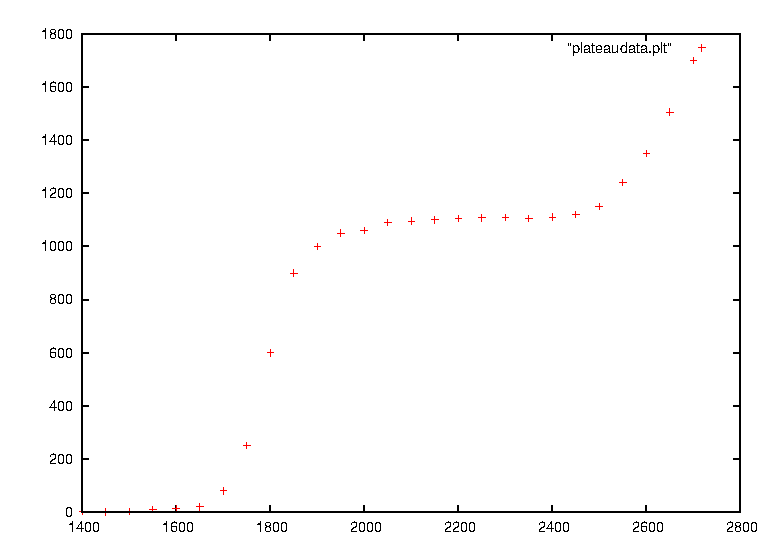
\includegraphics[width = 75mm]{./picture/plateaugnuplot.eps}
   \end{center}
   \caption{\texttt{plateaudata.plt}をgnuplotを用いて描いた時の様子。}
   \label{Fig:plateaugnuplot}
  \end{minipage}
  \begin{minipage}{0.53\hsize}
   \begin{center}
    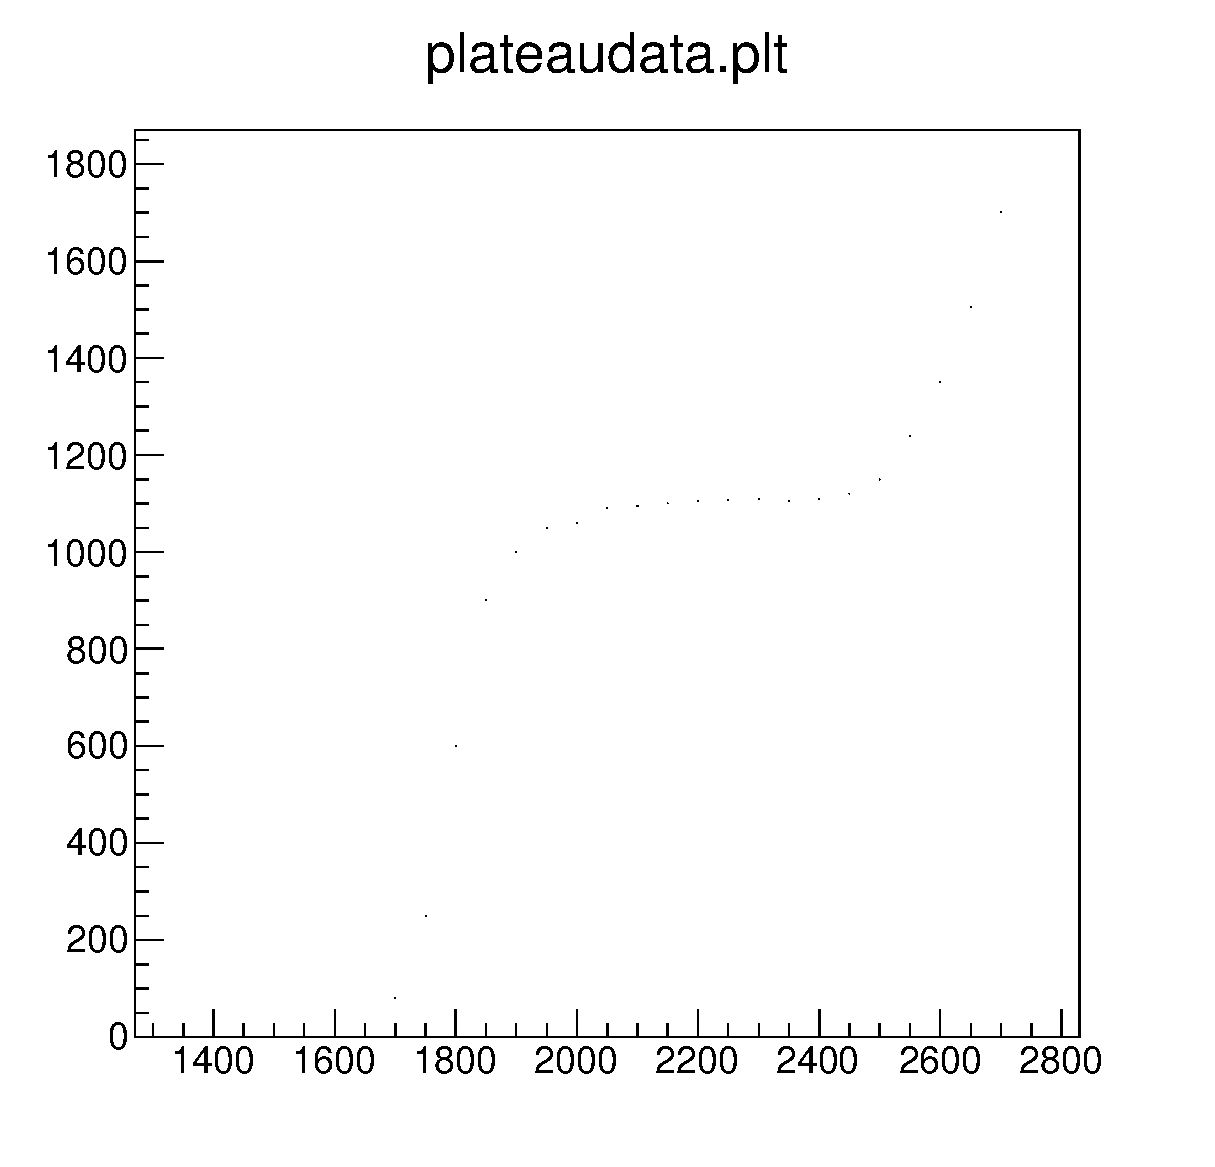
\includegraphics[width = 75mm]{./picture/plateaucanvas1.eps}
   \end{center}
   \caption{\texttt{plateaudata.plt}を\texttt{plateauplot.cpp}を用いて描いた時の様子。}
   \label{Fig:plateaucanvas1}
  \end{minipage}
 \end{figure}
 
 これを\ROOT で行う最低限のサンプルプログラムを示す。
  \begin{itembox}{\texttt{plateauplot.cpp}}
\begin{verbatim}
#include "TGraph.h"
#include "TCanvas.h"

TCanvas *plateauplot(){
  TCanvas *c1 = new TCanvas("c1", "c1", 600, 600) ;
  TGraph *f = new TGraph("plateaudata.plt", "%lf %lf") ;
  f->Draw("AP") ;
  return c1 ;
}
\end{verbatim}
  \end{itembox}
  この実行結果が図\ref{Fig:plateaucanvas1}である。
  
  
   \subsubsection{練習}
   
\begin{enumerate}
 \item プログラムの各行を理解せよ。
   \begin{description}
    \item[ヒント] \url{http://root.cern.ch/root/html/TGraph.html}
    \item[ヒント] \url{http://root.cern.ch/root/html/TGraph.html#TGraph:TGraph@10}
    \item[ヒント] \url{http://root.cern.ch/root/html/TGraph.html#TGraph:Draw}
    \item[ヒント] \url{http://root.cern.ch/root/html/TGraphPainter.html}
   \end{description}
       
 \item 引数をデータファイル名にするように変更せよ。
 \item 図\ref{Fig:plateaucanvas1}を見てわかるように、
       デフォルトではマーカーのサイズが小さい。
       マーカーサイズを調整したり、
       軸のタイトルを変更するなどしておしゃれせよ。
   \begin{description}
    \item[ヒント] \url{http://root.cern.ch/root/html/TAttMarker.html#TAttMarker:SetMarkerStyle}
    \item[ヒント] \url{http://root.cern.ch/root/html/TAttMarker.html#TAttMarker:SetMarkerSize}
    \item[ヒント] \url{http://root.cern.ch/root/html/TAttMarker.html#TAttMarker:SetMarkerColor}
    \item[ヒント] \url{http://root.cern.ch/root/html/TAttPad.html#TAttPad:SetLeftMargin}
   \end{description}
\end{enumerate}
   
   
   \subsubsection{解答例}

\begin{enumerate}
 \item プログラムの各行を理解せよ。
 \item 引数をデータファイル名にするように変更せよ。
 \item 図\ref{Fig:plateaucanvas1}を見てわかるように、
       デフォルトではマーカーのサイズが小さい。
       マーカーサイズを調整したり、
       軸のタイトルを変更するなどしておしゃれせよ。
         \begin{itembox}{\texttt{plateauplotsol1.cpp}}
\begin{verbatim}
...
TCanvas *plateauplotsol1(char *datafilename)){
  TCanvas *c1 = new TCanvas("c1", "c1", 600, 600) ;
  c1->SetGrid(1,1) ;
  c1->SetLogy() ;
  c1->SetLeftMargin(0.14) ;
  TGraph *f = new TGraph(datafilename, "%lf %lf") ;
  f->SetMarkerStyle(20) ;
  f->SetMarkerSize(1.1) ;
  f->SetMarkerColor(kRed) ;
  f->SetTitle("Plateau Curve") ;
  f->GetXaxis()->SetTitle("Voltage[V]") ;
  f->GetYaxis()->SetTitle("Counts[c/min]") ;
  f->GetYaxis()->SetTitleOffset(1.4) ;
  f->Draw("AP") ;
  return c1 ;
}
\end{verbatim}
  \end{itembox}
\begin{figure}[htbp]
   \begin{center}
    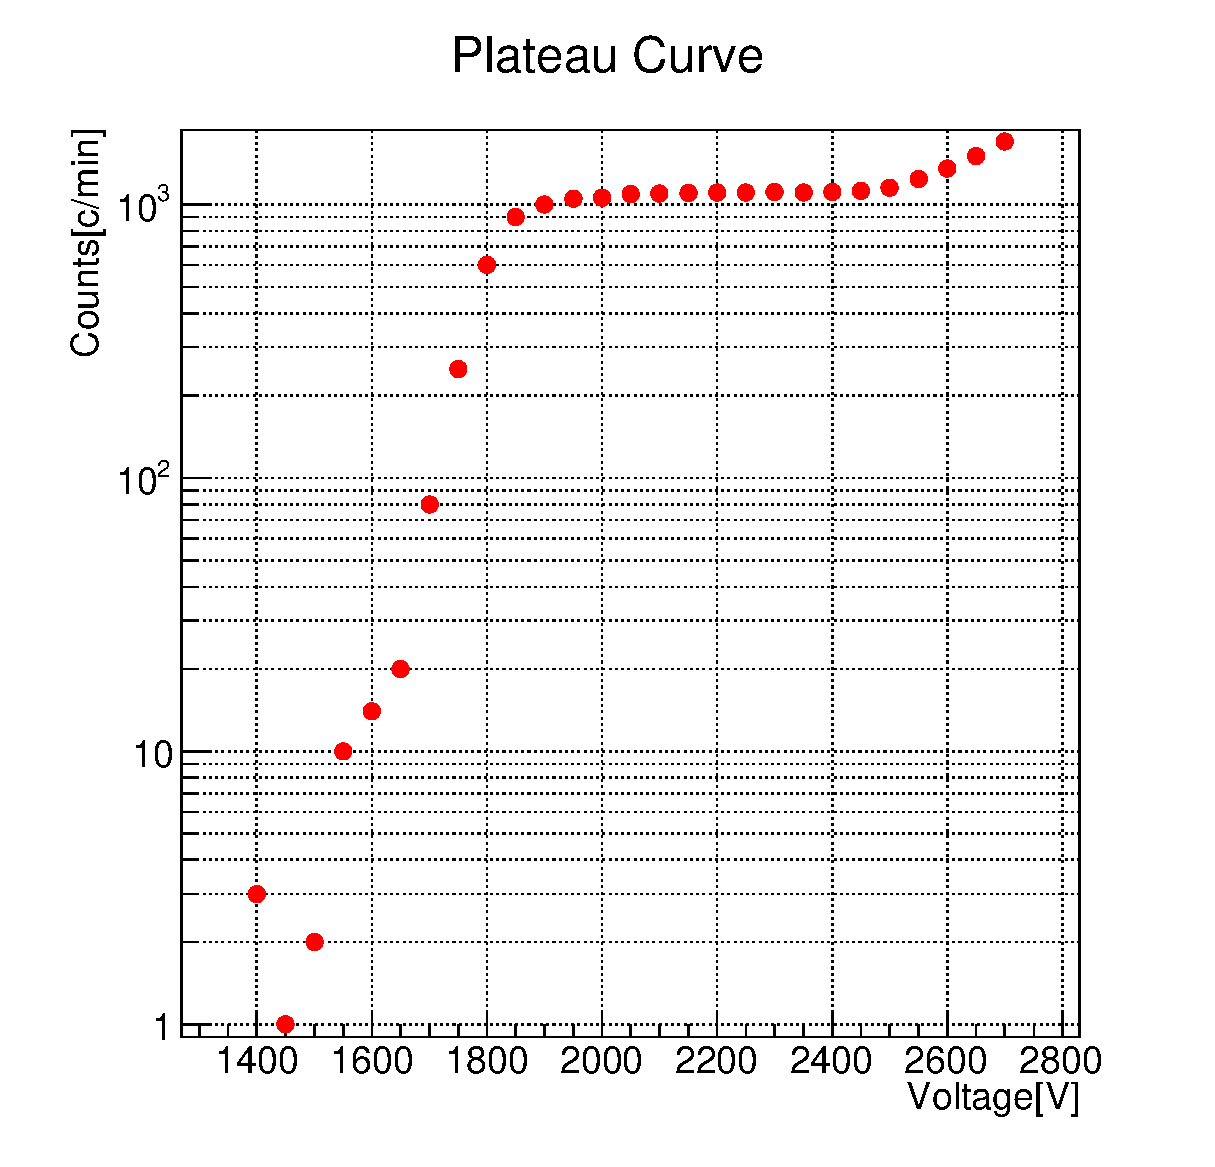
\includegraphics[width = 75mm]{./picture/plateaucanvas2.eps}
   \end{center}
   \caption{\texttt{plateauplotsol1.cpp}の実行結果。}
   \label{Fig:plateaucanvas2}
\end{figure}
\end{enumerate}



 
 
\subsection{ランダムウォーク}
 \begin{itembox}{\texttt{randomwalk.cpp}}
\begin{verbatim}
#include "TRandom3.h"
#include "TCanvas.h"
#include "TGraph.h"

TCanvas *randomwalk(){
  const int imax = 100 ;
  double x[imax] = {0.} ;
  double y[imax] = {0.} ;

  TRandom3 RandomGenerator(unsigned(time(NULL))) ;
  TCanvas *c1 = new TCanvas("c1", "c1", 600,600) ;
  c1->SetGrid(1,1) ;  
  for(int i = 1 ; i < imax ;i++){
    x[i] = RandomGenerator.Uniform(-1., 1.) + x[i-1] ; // 前の位置から[-1,1]だけx座標を移動
    y[i] = RandomGenerator.Uniform(-1., 1.) + y[i-1] ; // 前の位置から[-1,1]だけy座標を移動
  }
  TGraph  *f  = new TGraph(imax, x, y) ;
  f->SetLineStyle(1) ;
  f->SetLineWidth(2) ;
  f->SetLineColor(kRed) ;
  f->SetMarkerStyle(20) ;
  f->SetMarkerSize(1.1) ;
  f->SetMarkerColor(kBlue) ;

  f->Draw("APL") ;
  return c1 ;
}
\end{verbatim}
  \end{itembox}
 \begin{figure}[htbp]
  \begin{center}
   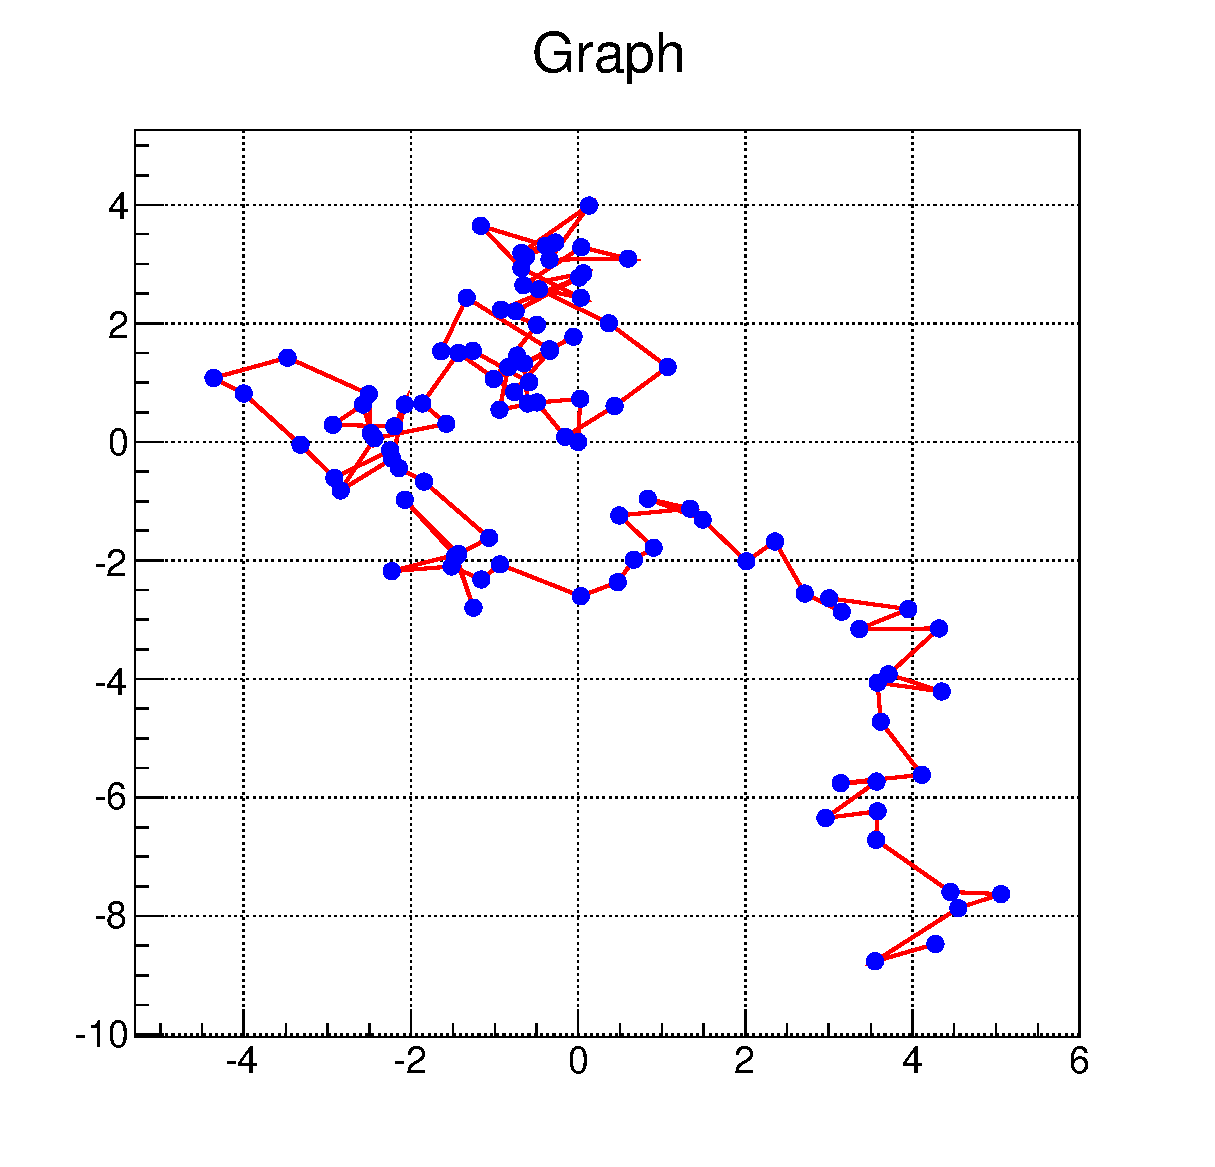
\includegraphics[width = 90mm]{./picture/randomwalkcanvas1.eps}
  \end{center}
  \caption{\texttt{randomwalk.cpp}の実行結果}
  \label{Fig:randomwalkcanvas1}
 \end{figure}

\subsubsection{練習}
\begin{enumerate}
 \item プログラムの各行を説明せよ
   \begin{description}
    \item[ヒント] \url{http://root.cern.ch/root/html/TGraph.html}
    \item[ヒント] \url{http://root.cern.ch/root/html/TGraph.html#TGraph:TGraph@2}
   \end{description}
 \item 今はx,yそれぞれの変化は[-1,1]で与えているが、
       現在位置から半径1の円周上が新しい点になるようにプログラムを変更せよ。
       これはTGraphの練習というよりも乱数の練習である。
   \begin{description}
    \item[ヒント] \url{http://root.cern.ch/root/htmldoc/TRandom.html#TRandom:Circle}
   \end{description}
       
\end{enumerate}

\subsubsection{解答例}

\begin{enumerate}
 \item プログラムの各行を説明せよ
 \item 今はx,yそれぞれの変化は[-1,1]で与えているが、
       現在位置から半径1の円周上が新しい点になるようにプログラムを変更せよ。
       \begin{itembox}{\texttt{randomwalksol1.cpp}}
\begin{verbatim}
...
TCanvas *randomwalksol1(){
  const int imax = 100 ;
  double x[imax] = {0.} ;
  double y[imax] = {0.} ;
  double deltax ;
  double deltay ;
  double radius = 1.0 ;
...
  for(int i = 1 ; i < imax ;i++){
    RandomGenerator.Circle(deltax, deltay, radius) ; // 半径radiusの円周上に一様に乱数を生成する。
    x[i] = deltax + x[i-1]; // 前の座標からdeltaxだけ移動する
    y[i] = deltay + y[i-1]; // 前の座標からdeltayだけ移動する
  }
  TGraph  *f  = new TGraph(imax, x, y) ;
...
\end{verbatim}
       \end{itembox}

\end{enumerate}
